\documentclass{article}

\usepackage[utf8]{inputenc}
%\usepackage[francais]{babel}
\usepackage[british,UKenglish,USenglish,english,american]{babel}
\usepackage[T1]{fontenc}
\usepackage{graphicx}
\usepackage{caption}
\usepackage{subcaption}
\usepackage{array}
\usepackage{amsmath}
\usepackage{amsthm}
\usepackage{amssymb}
\usepackage{amsfonts}
\usepackage{amsopn}
\usepackage[usenames,dvipsnames]{color}
\usepackage[left=3.3cm,right=3.3cm,top=3.3cm,bottom=3.3cm]{geometry}

\usepackage{multicol}
\usepackage[framemethod=tikz]{mdframed}
\tikzstyle{vertex}=[circle,fill=black!25,minimum size=20pt,inner sep=0pt]
\tikzstyle{edge} = [draw,thick,->]
\tikzstyle{weight} = [font=\small]
\usetikzlibrary{arrows}
\usepackage{listings}
\definecolor{gray}{rgb}{0.7,0.7,0.7}
\definecolor{dkgreen}{rgb}{0.25,0.7,0.35}
\definecolor{dkred}{rgb}{0.7,0,0} 
\lstset{language=Python,numbers=left,numberstyle=\tiny\color{gray},basicstyle=\rm\footnotesize,keywordstyle=\bfseries\color{dkred},frame=single,commentstyle=\color{gray}=small, stringstyle=\color{dkgreen}}
\newenvironment{changemargin}[2]{\begin{list}{}{%
\setlength{\topsep}{0pt}%
\setlength{\leftmargin}{0pt}%
\setlength{\rightmargin}{0pt}%
\setlength{\listparindent}{\parindent}%
\setlength{\itemindent}{\parindent}%
\setlength{\parsep}{0pt plus 1pt}%
\addtolength{\leftmargin}{#1}%
\addtolength{\rightmargin}{#2}%
}\item }{\end{list}}

\title{Lab $2$: Support Vector Machines\\
\large{DD2431 - Machine Learning}}
\date{\today}
\author{Mélanie Sedda, Pierre Springer}

\begin{document}
\maketitle

\section{Linear classifier}
The goal of a linear classifier is to find a vector $w$ such that all the points of the first class ($t = 1$) are such that $w^Tx \geq 0$ and all the points of the second class ($t = -1$) are such that $w^Tx \leq 0$ . The hyperplane $w^Tx = 0$ is the boundary between the two classes.\\

We can notice that multiplying $w$ by some constant doesn't change the classifier. So an equivalent problem is to say that we want $w^Tx \geq 1$ for the points such that $t = 1$ and $w^Tx \leq -1$ for the points such that $t = -1$ (we just need to scale $w$) which can be summarized in the equation $$tw^tx \geq 1.$$ 

\section{Maximal margin}
If several boundaries satisfy this property, we would like to find the best one. The best one is defined as the one that has the bigger margin, where the margin is the distance between the separating hyperplane and the closest point to it. If some points $p$ and $q$ are such that $w^Tp = 1$ and $w^Tq = -1$ then the projection of the length of the vector $p-q$ on the axis perpendicular to the plane must be equal to $2d$ since both $p$ and $q$ are at distance $d$ from the hyperplane. We can then write
$$2d = \frac{w^T(p-q)}{||w||} = \frac{w^Tp-w^Tq}{||w||} = \frac{2}{||w||}$$
and see that maximizing $d$ is equivalent to minimizing $||w||$.\\

So if we want to find the best linear classifier we need to solve the following optimization problem
\begin{align*}
\min_{w}\quad &||w|| \\
&t_iw^Tx_i \geq 1 \quad \forall i
\end{align*}
which can also be written as
\begin{align}
\min_{w}\quad &\frac{1}{2} w^Tw \\
&t_iw^Tx_i \geq 1 \quad \forall i  \nonumber.
\label{primal}
\end{align}

\section{Non-linear classifier}
If we want to create a non-linear classifier a trick is to transform the input data. So instead of consider $x$ we will consider $\phi(x)$ for some function $\phi$ and we will try to separate these values linearly.

\section{Kernel trick}
If $\phi$ maps the points into a very high dimensional space, we intuitively feel that the chance that the problem becomes linearly separable are higher (actually if we have as many dimensions as points, the problem is always linearly separable because we can simply use the first dimension to separate one point from the others, then the second one to separate another point from the remaining ones, etc). The kernel trick is to utilize the advantages of a high-dimensional space without actually representing anything high-dimensional. For this, we need that the only operation done in the high-dimensional space is to compute scalar products between pairs of items. The trick is then to express the scalar product in the high dimensional space in function of the original (low-dimensional) representation, i.e.
$$\phi(x) \cdot \phi(y) = \mathcal{K}(x,y).$$
The function $\mathcal{K}$ is called a kernel. So kernels are functions that correspond to a scalar product is some high dimensional space.\\

Common kernels are
\paragraph{Linear kernel}
$$\mathcal{K}(x,y) = x \cdot y + 1$$
\paragraph{Polynomial kernel}
$$\mathcal{K}(x,y) = (x \cdot y + 1)^p$$
\paragraph{RBF kernel}
$$\mathcal{K}(x,y) = e^{-\frac{||x-y||^2}{2\sigma^2}}$$
\paragraph{Sigmoid kernel}
$$\mathcal{K}(x,y)  = \tanh(k x \cdot y - \delta)$$
Then additional $+1$ terms are here to allow hyperplanes with a bias, i.e. that that do not necessarily contain the origin.\\

But how do we make some scalar products appear? For this, we will consider the dual problem of (\ref{primal}). There are as many dual variables as primal constraints. Let us call $\alpha_i$ those variables. The constraints on these variables are simply $\alpha_i \geq 0$ and the objective becomes
$$\max_{\alpha} \ \min_{w} \ L = \max_{\alpha} \ \min_{w} \ \frac{1}{2} w^Tw - \sum_i \alpha_i (t_iw^T\phi(x_i)-1).$$ 
Since
$$\frac{\partial L}{\partial w} = w - \sum_i \alpha_i t_i \phi(x_i)$$
the $w$ that minimizes L is
$$w = \sum_i \alpha_i t_i \phi(x_i),$$
$$ \min_{w} \ L = \frac{1}{2} \sum_{i,j} \alpha_i \alpha_j t_i t_j \phi(x_i)^T \phi(x_j) - \sum_{i,j} \alpha_i \alpha_j t_i t_j \phi(x_i)^T \phi(x_j) + \sum_i \alpha_i$$
and the dual problem is
 \begin{align*}
\max_{\alpha} \ &\sum_i \alpha_i -  \frac{1}{2} \sum_{i,j} \alpha_i \alpha_j t_i t_j \phi(x_i)^T \phi(x_j)\\
&\alpha_i \geq 0 \quad \forall i  \nonumber.
\end{align*}
We see that we indeed only have a scalar in the high dimensional space and it can be replaced by a kernel function. We can also express this problem is a more compact form using vectors and matrices. The canonical form of the dual problem is 
 \begin{align}
\min_{\alpha} \ & \frac{1}{2} \alpha^T P \alpha - \alpha \cdot e\\
&\alpha \geq 0  \nonumber.
\label{dual}
\end{align}
where $P_{i,j} = t_it_j\mathcal{K}(x_i, x_j)$.

\section{Slack variables}
Even if the problem is not separable, we could want to find a reasonable boundary. We allow some points to be misclassified but we had a penalty in that case.
The primal problem can then be formulated as
\begin{align}
\min_{w}\quad &\frac{1}{2} w^Tw + C \sum_i \xi_i \\
&t_iw^Tx_i \geq 1- \xi_i \quad \forall i  \nonumber.
\label{primalslack}
\end{align}
where the $\xi_i$ are called slack variables and the dual problem becomes
 \begin{align}
\min_{\alpha} \ & \frac{1}{2} \alpha^T P \alpha - \alpha \cdot e\\
&0 \leq \alpha \leq C  \nonumber.
\label{dualslack}
\end{align}
with the same $P$ as before. $C$ is a parameter that can be tuned. If $C$ is large, then the misclassifications are highly penalized.

\section{Implementation in Python}
\lstinputlisting[caption=svm.py]{../codes/svm.py}
\lstinputlisting[caption=kernels.py]{../codes/kernels.py}

\section{Results}
\newpage
\subsection{Linear kernel}
\begin{figure}[!h]
	\begin{center}
		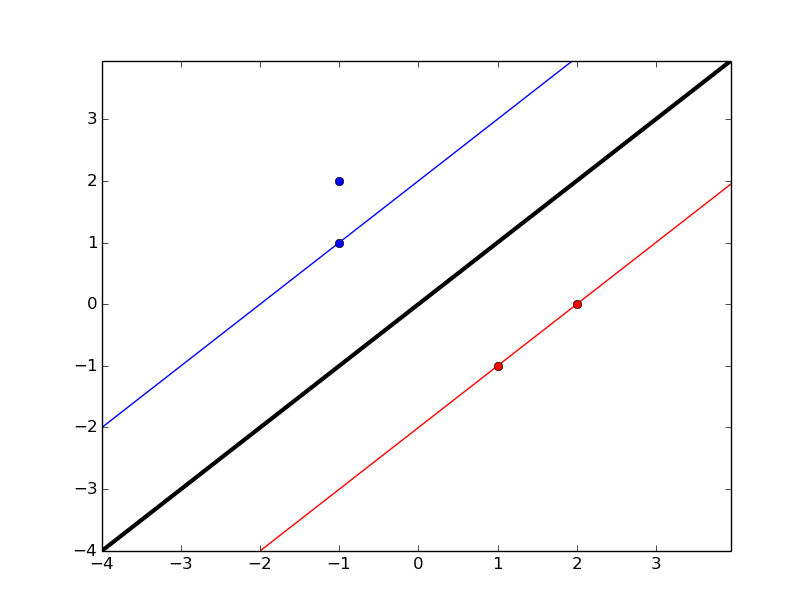
\includegraphics[width=10cm]{images/linear/figure_1.png}
		\caption{Linear kernel : test 1}
		\label{linear_figure_1}
	\end{center}
\end{figure}

\begin{figure}[!h]
	\begin{center}
		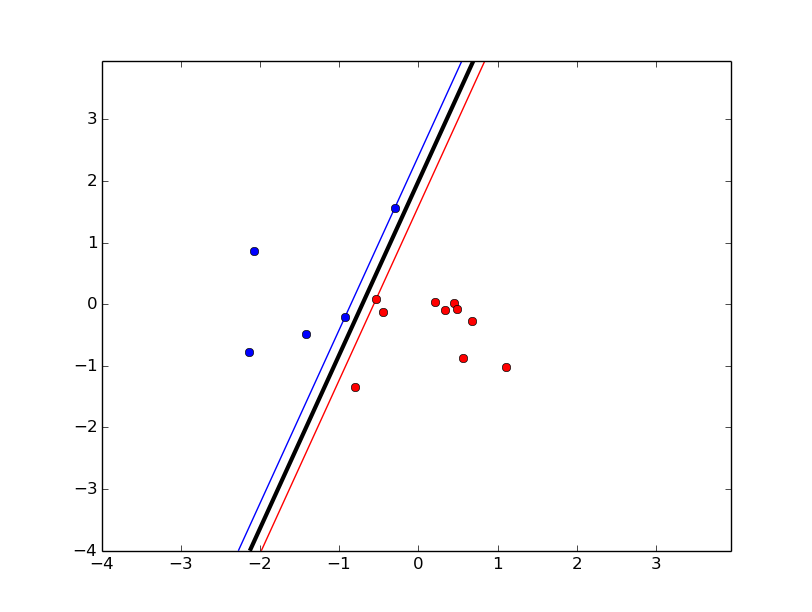
\includegraphics[width=10cm]{images/linear/figure_2.png}
		\caption{Test 2}
		\label{Linear kernel : test 2}
	\end{center}
\end{figure}

\newpage
\subsection{Polynomial kernel}
\begin{figure}[!h]
    \centering
    \begin{subfigure}[b]{0.3\textwidth}
        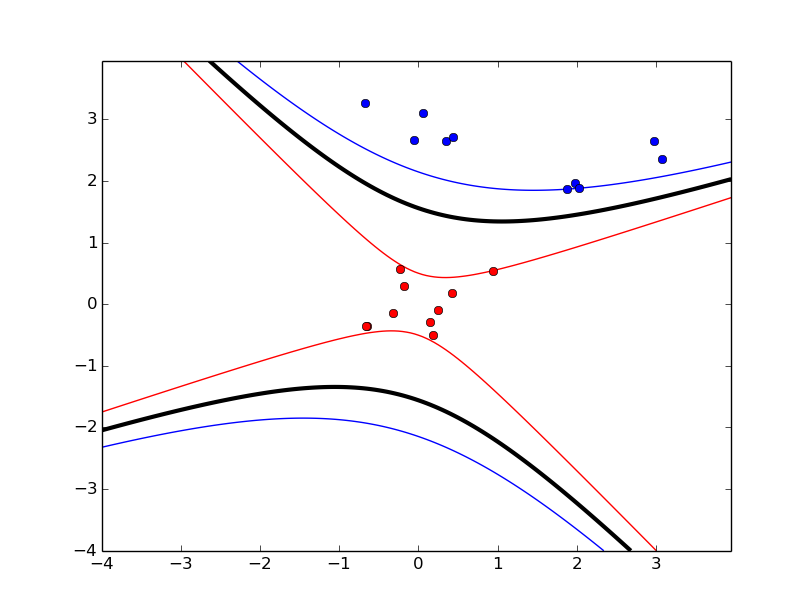
\includegraphics[width=1.2\textwidth]{images/pol/1/figure_2.png}
        \caption{$p = 2$} \label{polynomial_1_figure_1}
    \end{subfigure}
    ~ 
    \begin{subfigure}[b]{0.3\textwidth}
        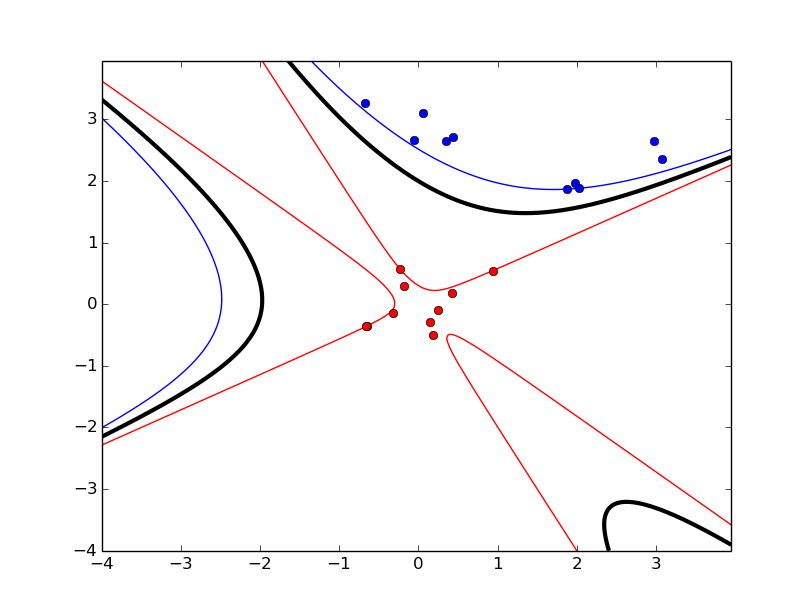
\includegraphics[width=1.2\textwidth]{images/pol/1/figure_3.png}
        \caption{$p = 3$}  \label{polynomial_1_figure_2}
    \end{subfigure}
     ~ 
    \begin{subfigure}[b]{0.3\textwidth}
        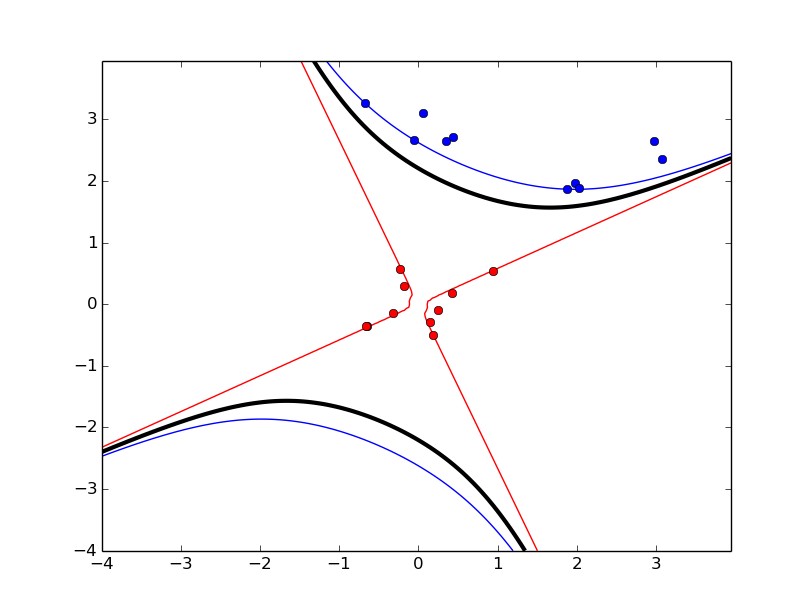
\includegraphics[width=1.2\textwidth]{images/pol/1/figure_4.png}
        \caption{$p = 4$}  \label{polynomial_1_figure_3}
    \end{subfigure}
    \caption{Polynomial kernel : test 1}
    \label{polynomial_1}
\end{figure}

\begin{figure}[!h]
    \centering
    \begin{subfigure}[b]{0.3\textwidth}
        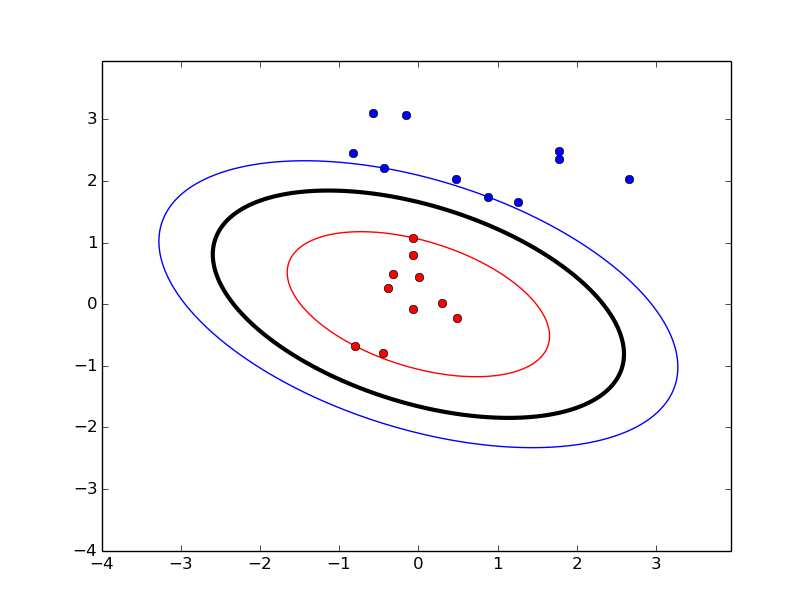
\includegraphics[width=1.2\textwidth]{images/pol/2/figure_2.png}
        \caption{$p = 2$} \label{polynomial_2_figure_1}
    \end{subfigure}
    ~ 
    \begin{subfigure}[b]{0.3\textwidth}
        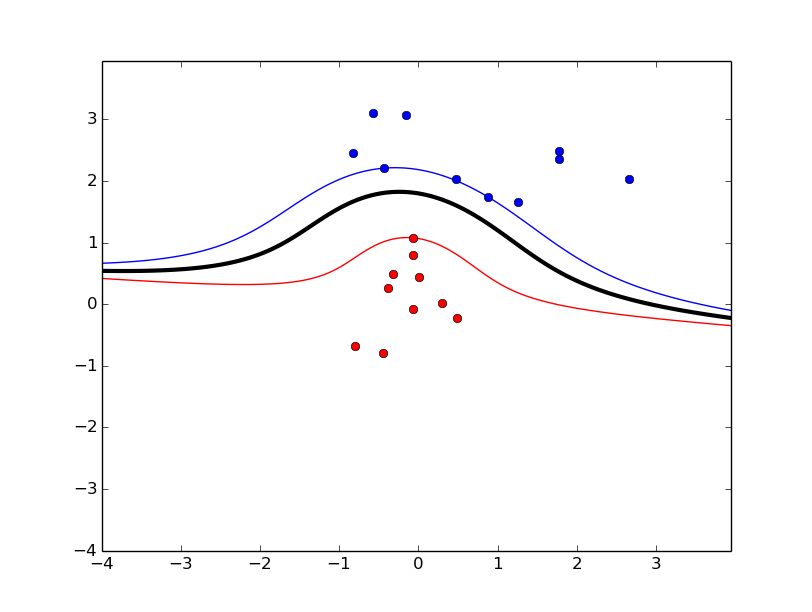
\includegraphics[width=1.2\textwidth]{images/pol/2/figure_3.png}
        \caption{$p = 3$}  \label{polynomial_2_figure_2}
    \end{subfigure}
     ~ 
    \begin{subfigure}[b]{0.3\textwidth}
        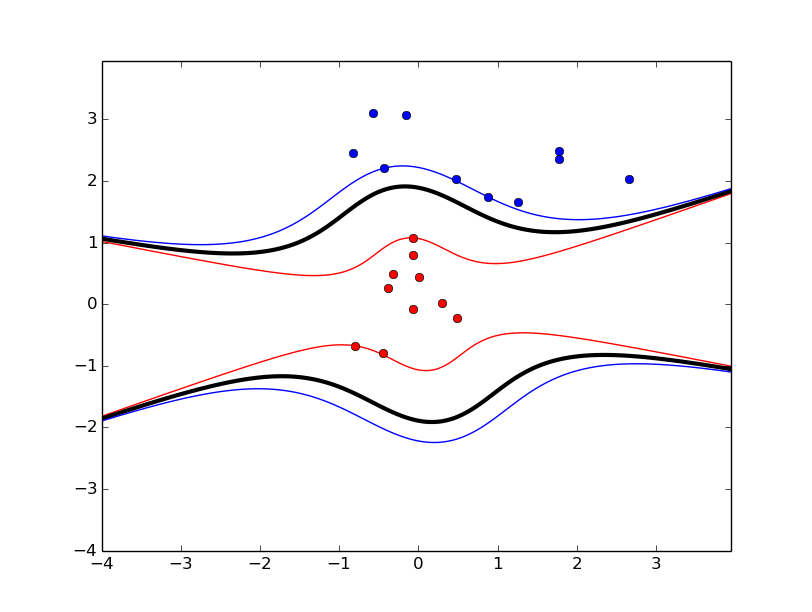
\includegraphics[width=1.2\textwidth]{images/pol/2/figure_4.png}
        \caption{$p = 4$}  \label{polynomial_2_figure_3}
    \end{subfigure}
    \caption{Polynomial kernel : test 2}
    \label{polynomial_2}
\end{figure}

\newpage
\subsection{RBF kernel}
\begin{figure}[!h]
    \centering
    \begin{subfigure}[b]{0.3\textwidth}
        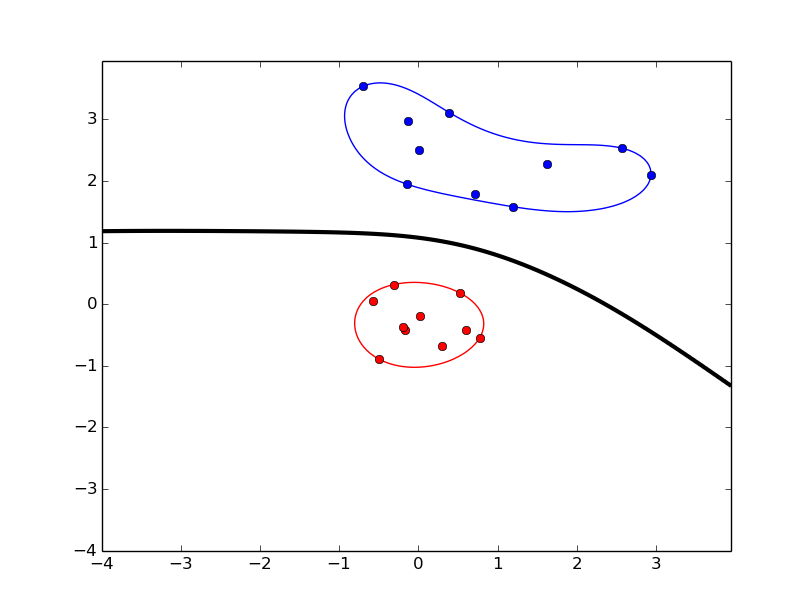
\includegraphics[width=1.2\textwidth]{images/rbf/1/figure_1.png}
        \caption{$\sigma = 1$} \label{rbf_1_figure_1}
    \end{subfigure}
    ~ 
    \begin{subfigure}[b]{0.3\textwidth}
        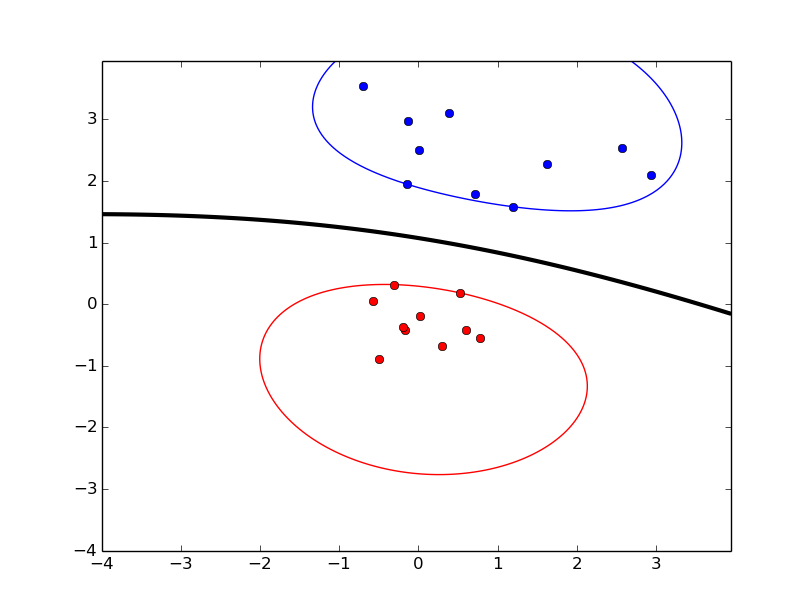
\includegraphics[width=1.2\textwidth]{images/rbf/1/figure_2.png}
        \caption{$\sigma = 2$}  \label{rbf_1_figure_2}
    \end{subfigure}
     ~ 
    \begin{subfigure}[b]{0.3\textwidth}
        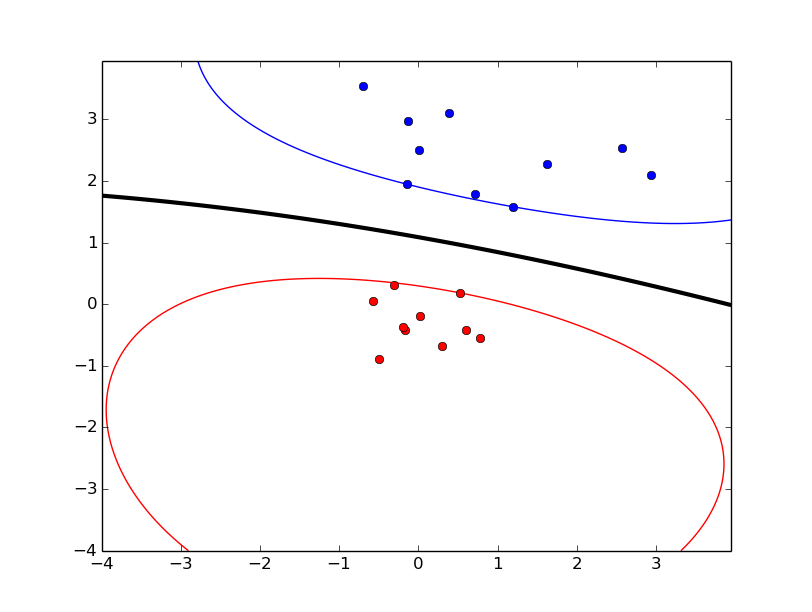
\includegraphics[width=1.2\textwidth]{images/rbf/1/figure_3.png}
        \caption{$\sigma = 3$}  \label{rbf_1_figure_3}
    \end{subfigure}
    \caption{RBF kernel : test 1}
    \label{rbf_1}
\end{figure}

\begin{figure}[!h]
    \centering
    \begin{subfigure}[b]{0.3\textwidth}
        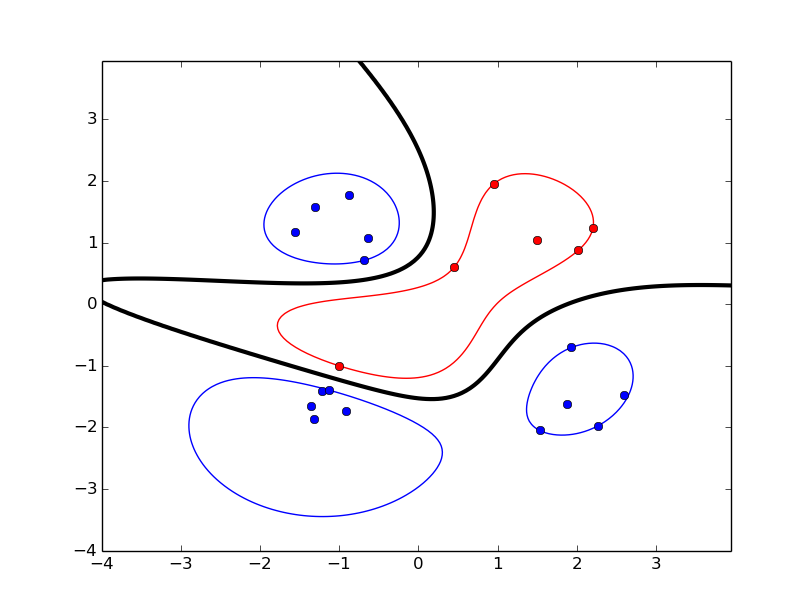
\includegraphics[width=1.2\textwidth]{images/rbf/2/figure_1.png}
        \caption{$\sigma = 1$} \label{rbf_2_figure_1}
    \end{subfigure}
    ~ 
    \begin{subfigure}[b]{0.3\textwidth}
        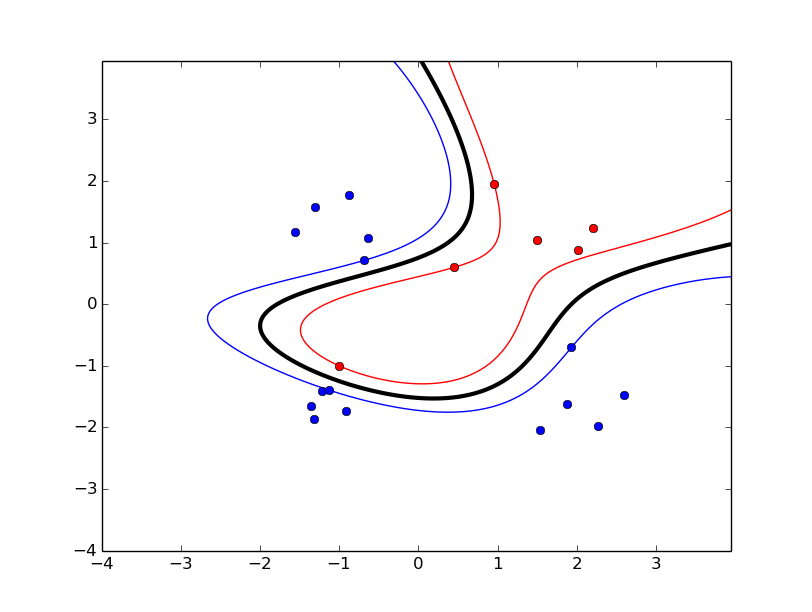
\includegraphics[width=1.2\textwidth]{images/rbf/2/figure_2.png}
        \caption{$\sigma = 2$}  \label{rbf_2_figure_2}
    \end{subfigure}
     ~ 
    \begin{subfigure}[b]{0.3\textwidth}
        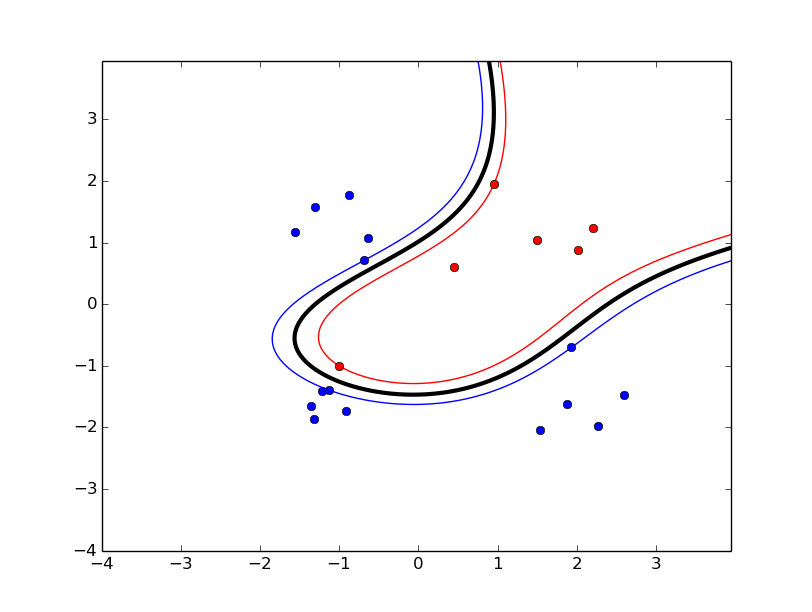
\includegraphics[width=1.2\textwidth]{images/rbf/2/figure_3.png}
        \caption{$\sigma = 3$}  \label{rbf_2_figure_3}
    \end{subfigure}
    \caption{RBF kernel : test 2}
    \label{rbf_2}
\end{figure}

\begin{figure}[!h]
    \centering
    \begin{subfigure}[b]{0.3\textwidth}
        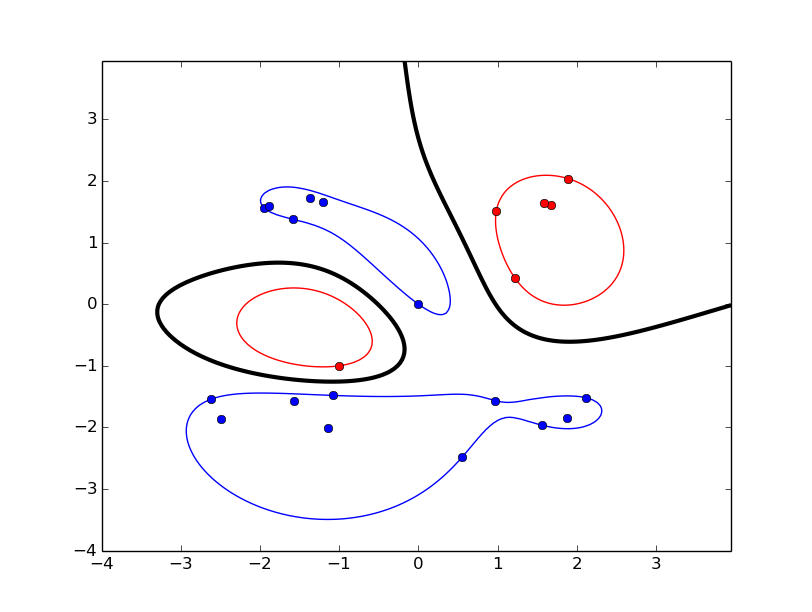
\includegraphics[width=1.2\textwidth]{images/rbf/3/figure_1.png}
        \caption{$\sigma = 1$} \label{rbf_3_figure_1}
    \end{subfigure}
    ~ 
    \begin{subfigure}[b]{0.3\textwidth}
        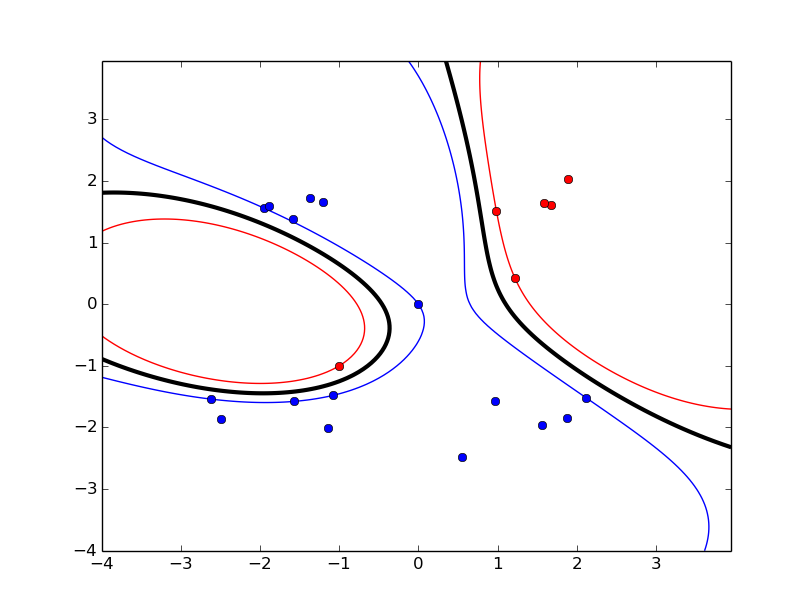
\includegraphics[width=1.2\textwidth]{images/rbf/3/figure_2.png}
        \caption{$\sigma = 2$}  \label{rbf_3_figure_2}
    \end{subfigure}
     ~ 
    \begin{subfigure}[b]{0.3\textwidth}
        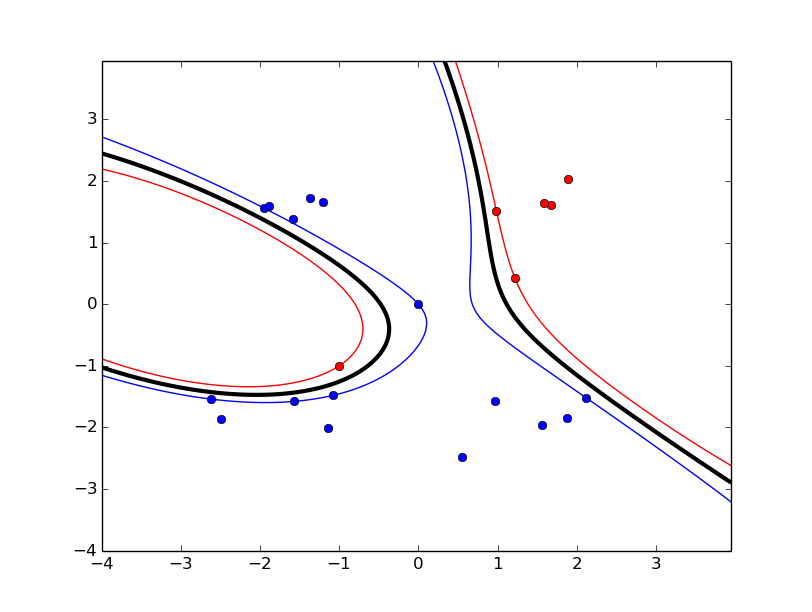
\includegraphics[width=1.2\textwidth]{images/rbf/3/figure_3.png}
        \caption{$\sigma = 3$}  \label{rbf_3_figure_3}
    \end{subfigure}
    \caption{RBF kernel : test 3}
    \label{rbf_3}
\end{figure}


The parameter $\sigma$ can be used to control the smoothness of the boundary.

\newpage
\subsection{Sigmoid kernel}
\begin{figure}[!h]
    \centering
    \begin{subfigure}[b]{0.3\textwidth}
        \includegraphics[width=1.2\textwidth]{images/sigmoid/test1_1.png}
        \caption{$k  = 0.1,~\delta = -5$} \label{sigmoid_1_figure_1}
    \end{subfigure}
    ~ 
    \begin{subfigure}[b]{0.3\textwidth}
        \includegraphics[width=1.2\textwidth]{images/sigmoid/test1_2.png}
        \caption{$k  = -0.1,~\delta = -2.5$}  \label{sigmoid_1_figure_2}
    \end{subfigure}
     ~ 
    \begin{subfigure}[b]{0.3\textwidth}
        \includegraphics[width=1.2\textwidth]{images/sigmoid/test1_3.png}
        \caption{$k  = 0.1,~\delta = 0.01$}  \label{sigmoid_1_figure_3}
    \end{subfigure}
    \caption{Sigmoid kernel : test 1}
    \label{rbf_1}
\end{figure}

\begin{figure}[!h]
    \centering
     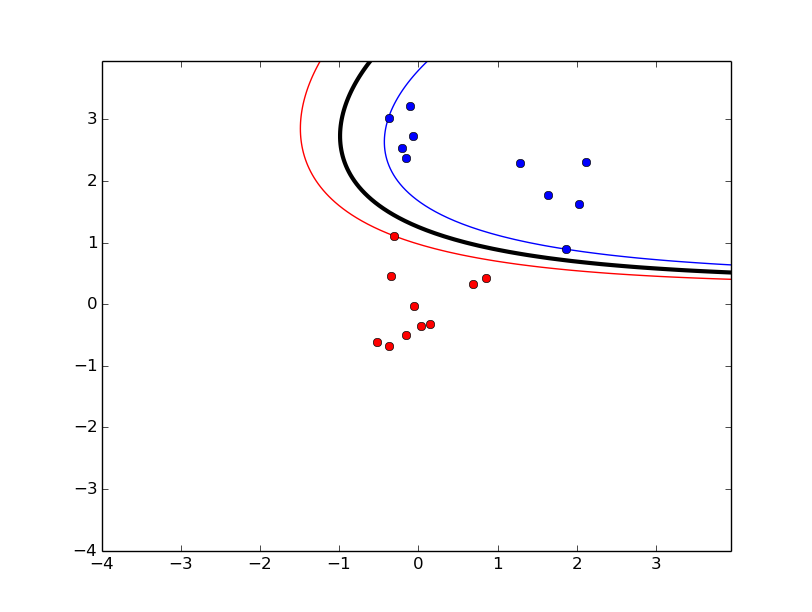
\includegraphics[width=0.8\textwidth]{images/sigmoid/sigmo2.png}

    \caption{Sigmoid kernel : test 2,$k  = 0.1,~\delta = -5$ }
    \label{rbf_2}
\end{figure}


As the $logh$ function has different numbers only close to 0, we see. that we can manipulate the scalar product to give it reasonable values with the factor $k$. To get this value close to 0, we can use the parameter $\delta$. A negative $k$ seems to invert the results and lead to worse ones.

\newpage

\subsection{Slack variables}
\begin{figure}[!h]
    \centering
    \begin{subfigure}[b]{0.35\textwidth}
        \includegraphics[width=1.2\textwidth]{images/slack/linCinf.png}
        \caption{$C = \inf$} \label{slack_lin_figure_1}
    \end{subfigure}
    ~ 
    \begin{subfigure}[b]{0.35\textwidth}
        \includegraphics[width=1.2\textwidth]{images/slack/linC4.png}
        \caption{$C = 4$}  \label{slack_lin_figure_2}
    \end{subfigure}
	\caption{Linear Kernel with slack-variable}
    \label{lin_slack}
\end{figure}

\begin{figure}[!h]
    \centering
 \begin{subfigure}[b]{0.35\textwidth}
        \includegraphics[width=1.2\textwidth]{images/slack/polyCinf.png}
        \caption{$C = \inf$}  \label{slack_poly_figure_1}
    \end{subfigure}
    \begin{subfigure}[b]{0.35\textwidth}
        \includegraphics[width=1.2\textwidth]{images/slack/polyC2.png}
        \caption{$C = 2$}  \label{slack_poly_figure_2}
    \end{subfigure}
	\caption{Polynomial Kernel with slack-variable}
    \label{lin_slack}
\end{figure}


\begin{figure}[!h]
    \centering
 \begin{subfigure}[b]{0.35\textwidth}
        \includegraphics[width=1.2\textwidth]{images/slack/RBFCinf.png}
        \caption{$C = \inf$}  \label{slack_rbf_figure_1}
    \end{subfigure}
    \begin{subfigure}[b]{0.35\textwidth}
        \includegraphics[width=1.2\textwidth]{images/slack/rbfwithC10.png}
        \caption{$C = 10$}  \label{slack_rbf_figure_2}
    \end{subfigure}
	\caption{RBF Kernel with slack-variable}
    \label{RBF_slack}
\end{figure}

\end{document}

